\section{SAD}
\subsection{Aufgabe}

%Aufgabenstellung
\begin{frame} %%Eine Folie
  \frametitle{Aufgabe} %%Folientitel

	\highlighton{Leitung des Teams Content \& Layout}
%   Auflistung mit Punkt davor
  	\begin{itemize}
   		\item Verteilung von Aufgaben
   		\item Fertigstellung des SAD-Dokuments
   		\item Kontrolle und Bewertung der Ergebnisse
  	\end{itemize}
	\bigskip \highlighton{Mitarbeit am SAD}
	\begin{itemize}
		\item Kontextdiagramm: Tutor
		\item Punkt F16: About us (Impressum)
		\item Punkt F17: Preismodell und Zahlungsinfos
		\item Punkt F19: Support und Kontaktdaten
		\item Abschnitt 3.4: Lehrer/Mentor zusammen mit Christian Dauerer
	\end{itemize}
\end{frame}

%\begin{frame} %%Eine Folie
%  \frametitle{Analyse} %%Folientitel
%
%  Um einen besseren Überblick zu Erhalten wurden die folgenden Fragen gestellt:
%  \bigskip
%% Aufzählung
%  \begin{enumerate}
%   \item Welche Grundanforderungen sind nötig?
%   \item Welcher Webserver steht zur Verfügung?
%   \item Welche Möglichkeiten gibt es zur Umsetzung?
%   \item Welche Sprachen werden benötigt?
%  \end{enumerate}
%
%\end{frame}

\subsection{Umsetzung}

%Kontext Tutor
\begin{frame}
  	\frametitle{Kontextdiagramm: Tutor} 
  
	\begin{tabular}{c|c}
	Ursprüngliche Version & Finale Version\\
	\hline
		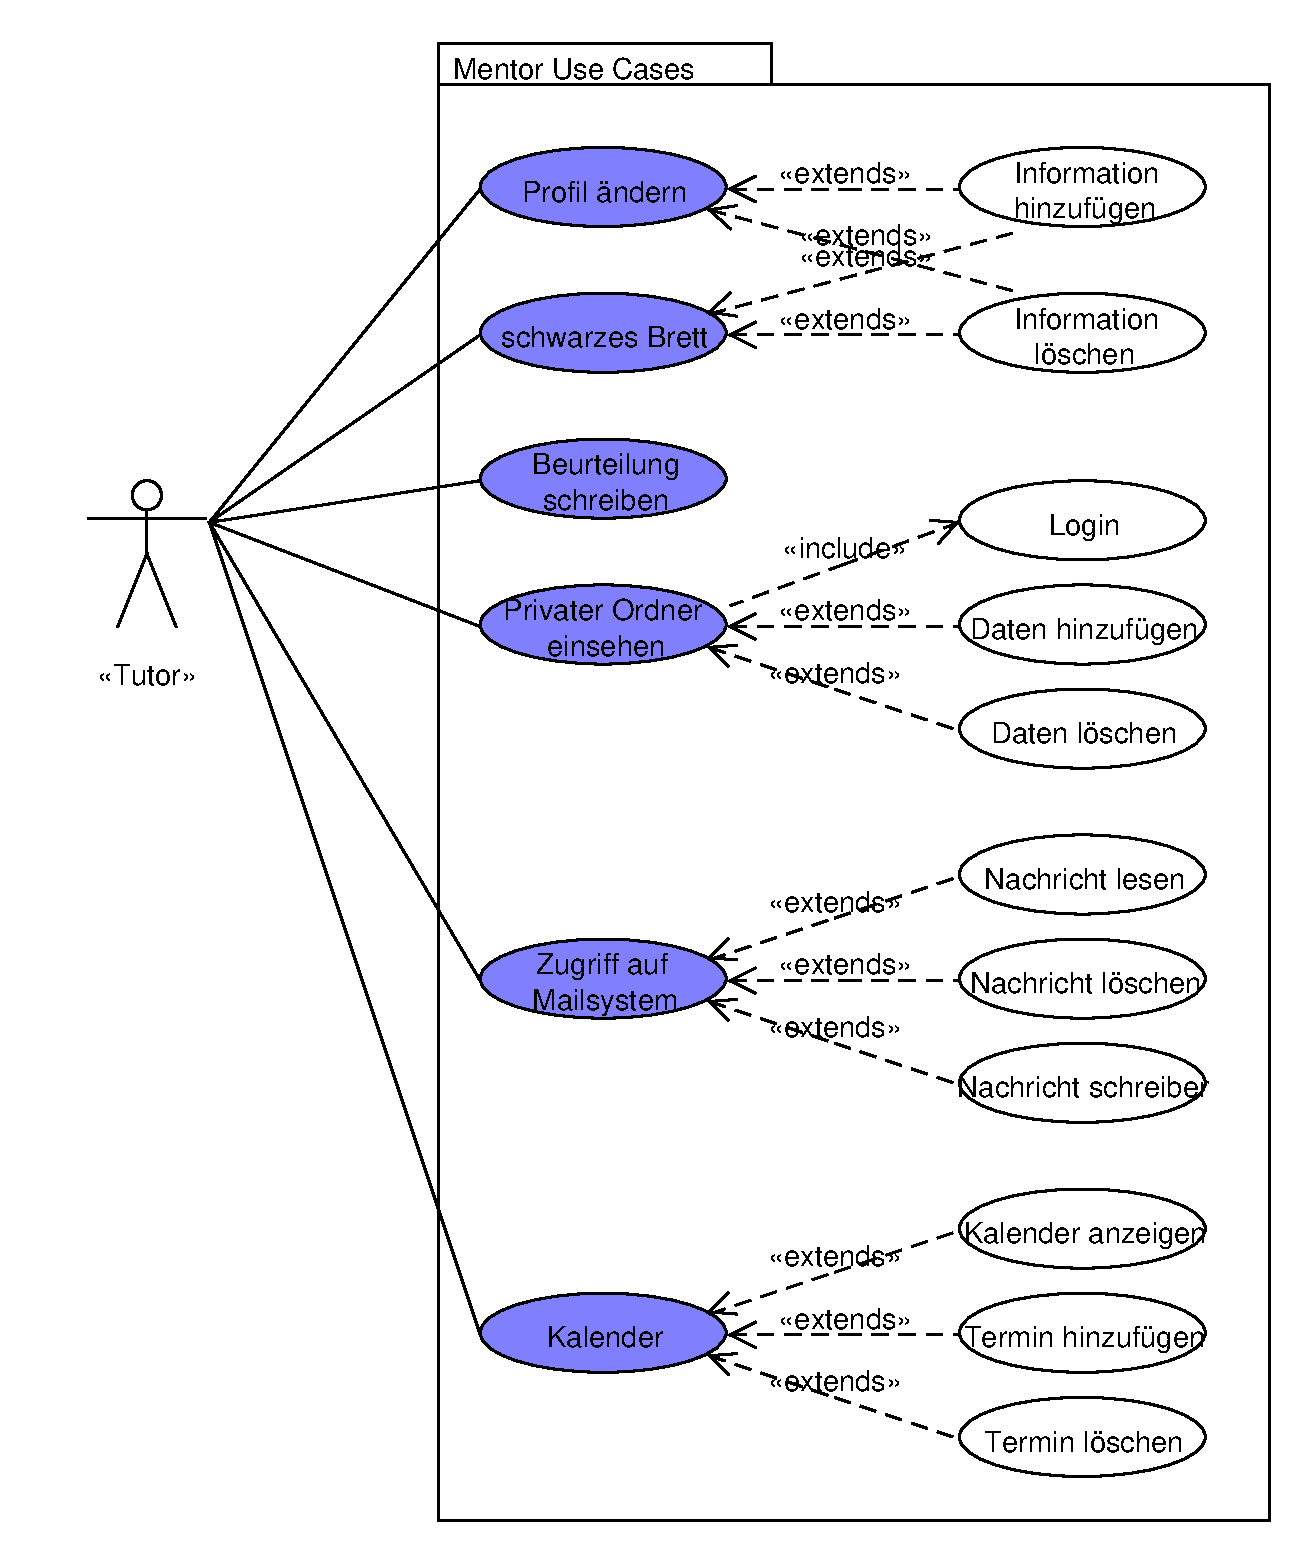
\includegraphics[width=0.5\linewidth]{./Source/UseCaseMentor_13.pdf}
		&
		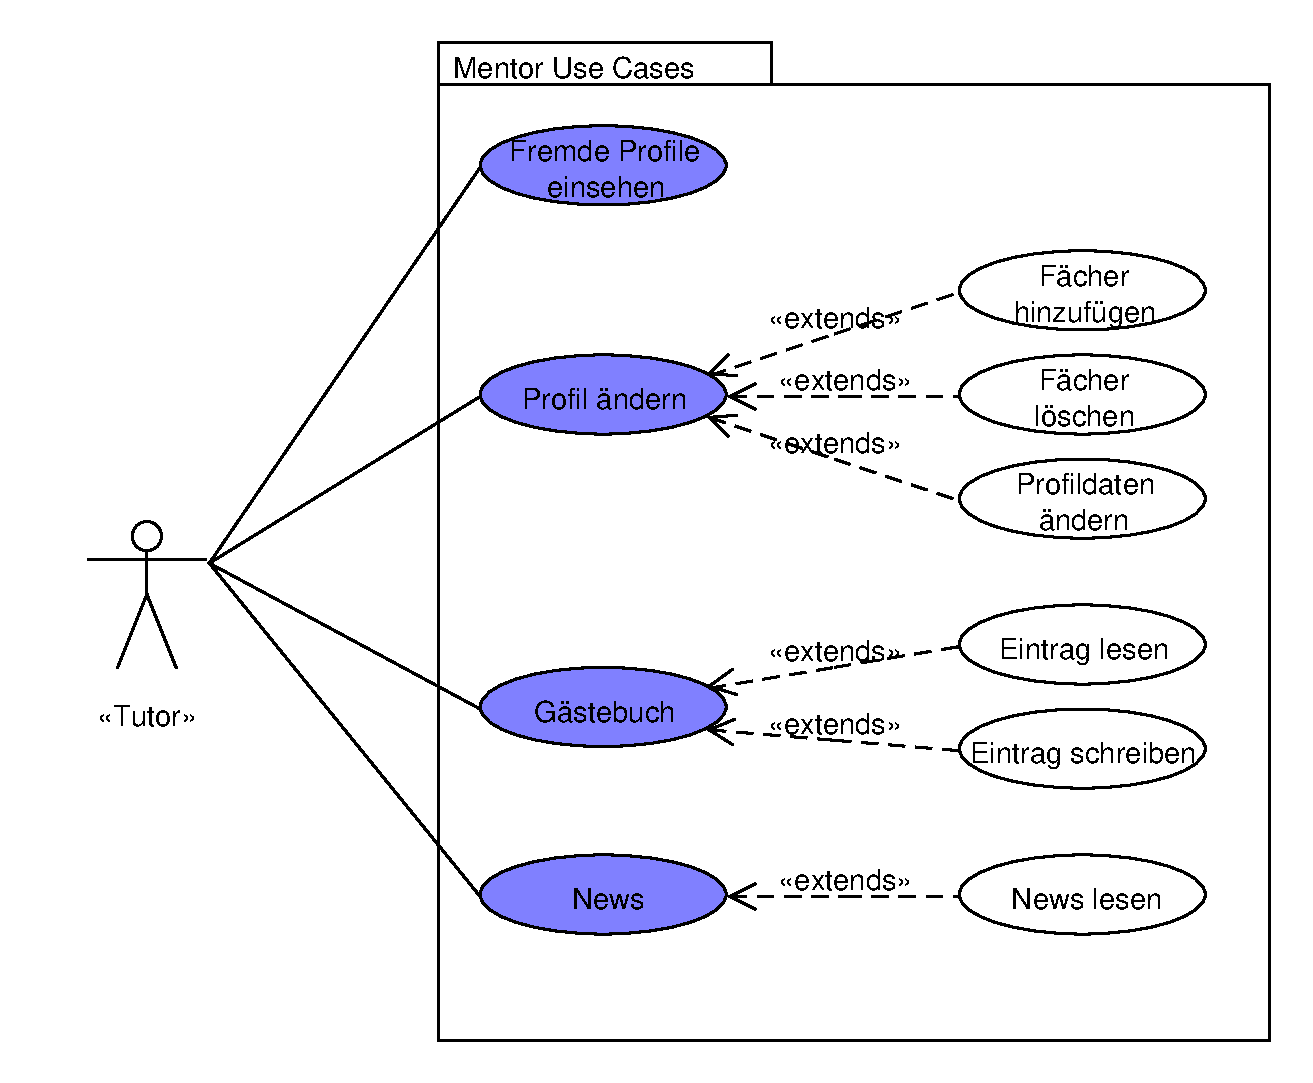
\includegraphics[width=.55\linewidth]{./Source/UseCaseMentor_14.pdf}
	\end{tabular}\\
\end{frame}

%Impressum
\begin{frame}
  	\frametitle{Punkt F16: About us(Impressum)} 
  
	Der Besucher der Webseite sollte die Möglichkeit haben, Informationen über Die Tutoren AG zu bekommen. Außerdem ist nach §5 Telemediengesetz (TMG) in Deutschland eine Impressumspflicht vorhanden.
	\bigskip\newline
	Das Impressum enthält:
	\begin{itemize}
		\item Firmenname
	  	\item Geschäftsführer (Inhaltlich Verantwortlicher, Vertretungsberechtigter)
		\item Anschrift der Die Tutoren AG (Straße, PLZ, Ort)
		\item Kontaktdaten (eMail, Telefon)
	\end{itemize}
\end{frame}

%Preismodell und Zahlungsinfos
\begin{frame}
  	\frametitle{Punkt F17: Zahlungsinformationen}
  
  	Der Besucher der Webseite sollte die Möglichkeit haben, sich vor der Anmeldung über verschiedenen Preismodelle und Arten der Zahlungsabwicklung zu informieren.
  	\bigskip\newline Dafür wurde eine eigene Seite mit statischen Inhalten geplant, welche den Besucher darüber informieren sollte.
\end{frame}

%Support und Kontaktdaten
\begin{frame}
  	\frametitle{Punkt F19: Support und Kontaktdaten}
  
  	Der Besucher der Webseite sollte die Möglichkeit haben, sich bei Fragen und Problemen an den Support der Die Tutoren AG zu wenden.
  	\bigskip\newline Dafür wurde die Seite "Kontakt" geplant. Diese soll statischen HTML Content beinhalten und ist über die Navigationsleiste zu erreichen.
\end{frame}

%Schwarzes Brett
\begin{frame}
  	\frametitle{Analyse - Schwarzes Brett}
  
	Eine geplante Funktion für den Tutor war ein schwarzes Brett, welches der Tutor für die Veröffentlichung von Informationen benutzen kann, wie z.B. eine Krankheitsmeldung oder neue Fächer usw. \newline
	Dafür wurde eingeplant:
	\begin{itemize}
		\item Eine DB-Tabelle für die Einträge
		\item Abfrage der Daten über SQL
		\item Weitergabe per JSON
		\item Anzeige über JavaScript
	\end{itemize}
	
\end{frame}

%Nachrichtensystem
\begin{frame}
 	\frametitle{Analyse - Nachrichtensystem}

	Eine geplante Funktion für den Tutor (wie für alle Benutzer) war ein systemweites Nachrichtensystem, damit Benutzer sich gegenseitig Nachrichten schicken können. \newline
	Dafür wurde eingeplant:
	\begin{itemize}
		\item Eine DB-Tabelle für die Einträge
		\item Abfragen der Daten über SQL
		\item Weitergabe per JSON
		\item Anzeige über jQuery
	\end{itemize}
	
\end{frame}
